\phantomsection
%\addcontentsline{toc}{chapter}{Introduzione}
\chapter{Introduzione}
\markboth{Introduzione}{}
% [titolo ridotto se non ci dovesse stare] {completo}

\section{Contesto applicativo} %\label{1sec:scopo}
Gli scacchi sono un gioco di strategia deterministico\footnote{Si definisce deterministico un gioco in cui gli stati assunti durante la partita sono determinati
unicamente dalle azioni dei giocatori, si parla quindi di giochi in cui non vi è una componente aleatoria.} a somma zero\footnote{Si definisce a somma zero un gioco in cui il guadagno o la perdita di un partecipante è perfettamente bilanciato da una perdita o un guadagno di un altro partecipante in una somma uguale e opposta.} e ad informazione completa\footnote{Si definisce ad informazione completa un gioco i cui stati sono
completamente espliciti ai giocatori, si parla quindi di giochi dove entrambi i giocatori hanno accesso a tutte le informazioni riguardanti lo stato della partita, non vi sono quindi "carte coperte" o elementi di sorpresa.}  
che si svolge su una tavola quadrata formata da 64 caselle, di due colori alternati,
detta scacchiera, sulla quale ogni giocatore contraddistinto da uno dei due colori (bianco o nero), dispone di 16 pezzi: un re, una regina, due alfieri, due cavalli, due torri e otto pedoni.
L'obiettivo del gioco è dare scacco matto, ovvero minacciare la cattura del re avversario mentre esso non
ha modo di rimuovere il re dalla sua posizione di pericolo alla sua prossima mossa.



\section{Motivazioni e obiettivi}
Gli scacchi, gioco nato in india attorno al 600 d.C. e campo di battaglia in uno dei più famosi scontri tra uomo e macchina\footnote{Nel 1996 e nel 1997 avvennero due delle partite di scacchi più importanti di sempre,
 per la prima volta un computer, Deep Blue progettato e prodotto da IBM, sfidava un campione del mondo di scacchi, e non un campione qualsiasi ma Garry Kasparov, uno dei giocatori più vincenti e titolati di sempre. 
 L'evento dalla notevole importanza mediatica terminò prima con una vittoria da parte di Kasparov nel 1996 e poi con una vittoria di Deep Blue in una rivincita del 1997, segnando per molti quella che rappresenta la
  fine della supremazia umana nel gioco degli scacchi. }, non hanno mai fallito nel saper cattivare  l'attenzione del grande pubblico nei loro 1400 anni di storia.
 \\È facile capire come sia possibile se ci si concentra su una delle caratteristiche fondamentali del 
<<<<<<< HEAD
 gioco degli scacchi  questa caratteristica è la \textbf{complessità}.\\In una partita di scacchi fin dalla prima mossa 
sono possibili 20 scelte, in quanto ognuno degli 8 pedoni del giocatore di partenza potrà essere mosso di una o due caselle ed ognuno dei due cavalli avrà 2 possibili mosse a disposizione, come visibile nella figura \ref{mosse}, per la seconda il totale di possibili combinazioni sale a 400, avendo il giocatore nero le stesse 20 mosse iniziali possibili in risposta ad ognuna delle 20 mosse del giocatore bianco.
 Dopo 5 mosse avremo 119,060,324 possibili risposte, frutto dell'elevato fattore di diramazione medio\footnote{ il fattore di diramazione medio è il numero medio di risposte possibili ad ogni mossa dell'avversario, negli scacchi, è stato calcolato che il fattore di diramazione medio sia compreso tra 28 e 35, ciò significa che, di media, un giocatore ha a disposizione circa 30 mosse legali ad ogni turno.} degli scacchi esteso per 5 mosse, in totale le possibili mosse di una partita si stimano attorno alle \(2^{155} \).
=======
 gioco degli scacchi: la \textbf{complessità}.\\In una partita di scacchi fin dalla prima mossa 
sono possibili 20 scelte, in quanto ognuno degli 8 pedoni del giocatore di partenza potrà essere mosso di una o due caselle ed ognuno dei due cavalli avrà 2 possibili mosse a disposizione, come visibile nella figura \ref{mosse}; per la seconda il totale di possibili combinazioni sale a 400, avendo il giocatore nero le stesse 20 mosse iniziali possibili in risposta ad ognuna delle 20 mosse del giocatore bianco,
 dopo 5 mosse avremo 119,060,324 possibili risposte, frutto dell'elevato fattore di diramazione medio\footnote{ Il fattore di diramazione medio è il numero medio di risposte possibili ad ogni mossa dell'avversario, negli scacchi. È stato calcolato che il fattore di diramazione medio sia compreso tra 28 e 35, ciò significa che, di media, un giocatore ha a disposizione circa 30 mosse legali ad ogni turno.} degli scacchi esteso per 5 mosse. In totale le possibili mosse di una partita si stimano attorno alle \(2^{155} \).
>>>>>>> ae51dff4cfbdc2ea8838854b1fb28749f0921b83
 \\Con uno spazio di ricerca cosi grande non dovrebbe stupire scoprire che è da quando esistono i computer che si cerca un modo
 di sfruttare la loro potenza di calcolo nel mondo degli scacchi.
 La nascita degli scacchi computazionali si deve al lavoro di Claude Shannon, famoso per i suoi innumerevoli contributi al 
 campo della teoria dell'informazione. Egli, con il suo paper "Programming a Computer for Playing Chess"\cite{shannon} del 1950 ha gettato le
 basi per quello che oggi è il campo conosciuto come scacchi computazionali.
 \\Questa tesi nasce dalla volontà di esplorare questo vasto e interessante campo dell'informatica e dal voler creare un testo
 in grado di guidare chiunque lo legga nella creazione di un motore scacchistico spiegando tutte le fasi della progettazione
 ed illustrando le possibili scelte che condizionano l'efficienza di un motore.


 \begin{figure}
    \centering
    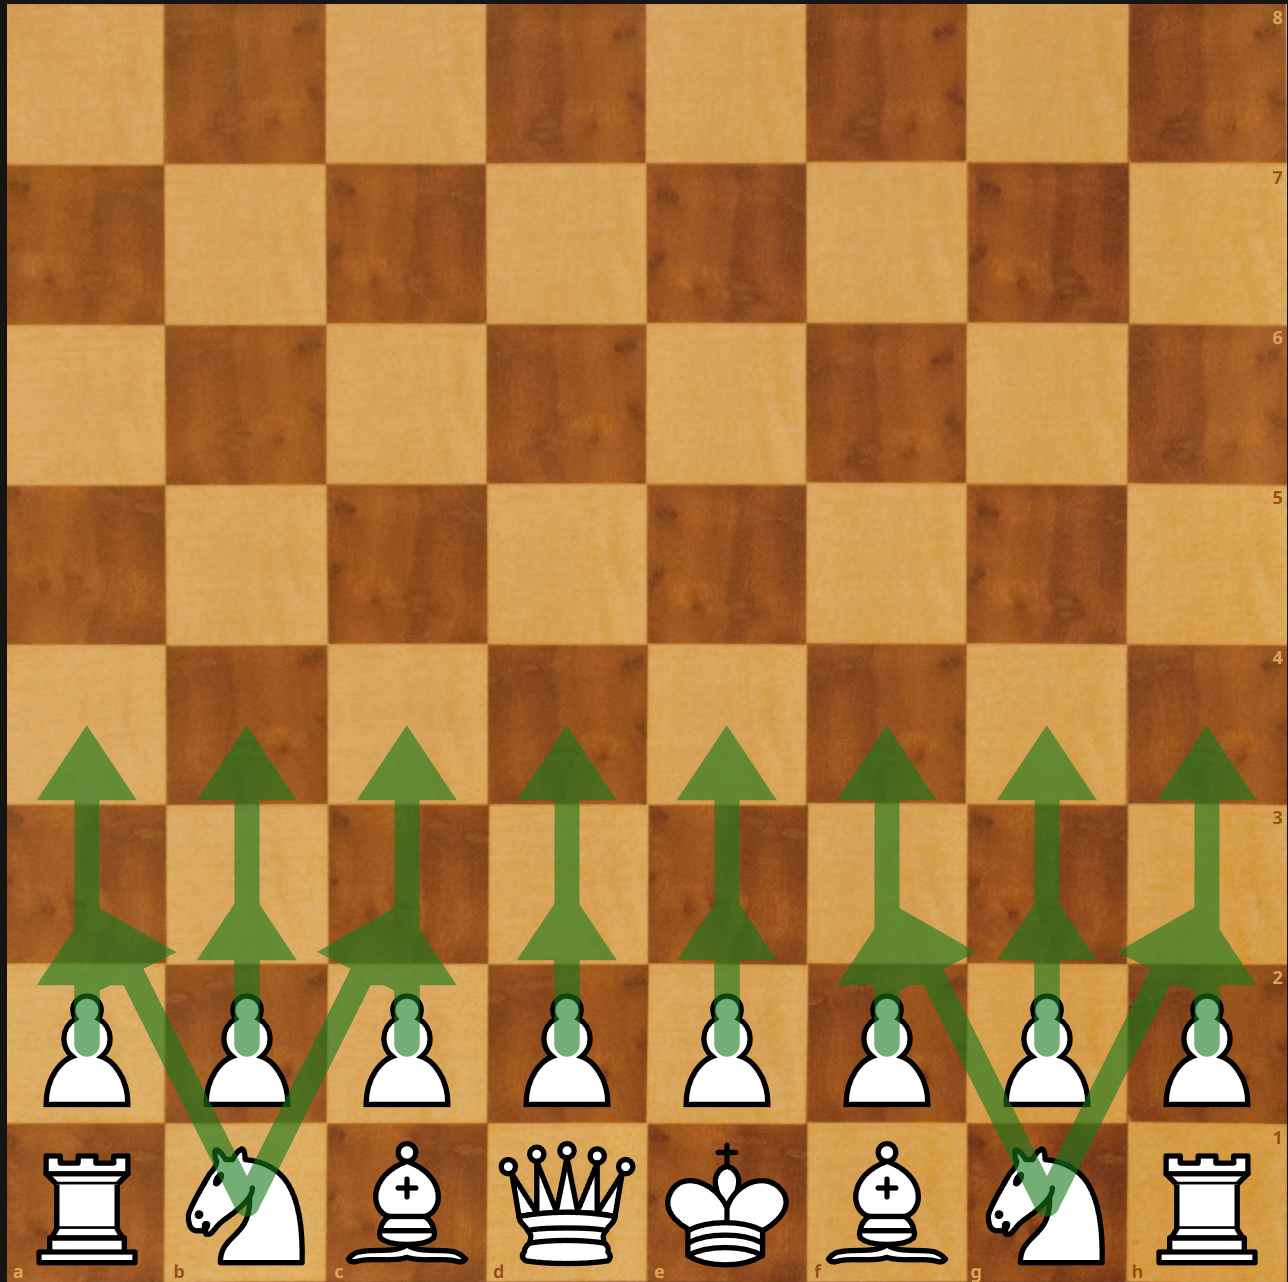
\includegraphics[width=\linewidth/2] {mosse.png}
    \caption{le 20 mosse iniziali possibili per il giocatore bianco ad inizio partita}
    \label{mosse}
\end{figure}






\section{Risultati ottenuti}
È stato ottenuto un motore scacchistico di medio livello che implementa tutte le componenti più importanti, in grado di essere 
capito da un novizio ma che allo stesso tempo funge da ottima base per lo sviluppo di un motore allo stato dell'arte e che riesce a confrontarsi e 
vincere in maniera convincente contro motori famosi per chi si approccia al mondo degli scacchi computazionali come Vice o TSCP; sono anche
stati raccolti dati sull'effetto di queste tecniche, utilizzati per produrre una prova della loro efficacia.



\section{Struttura della tesi}
La tesi è strutturata in 5 capitoli:
\begin{itemize}
\item Il primo funge da introduzione ed illustra a grandi linee il contenuto della tesi. 
\item Nel secondo viene affrontato il processo di progettazione di un motore scacchistico dal punto di vista teorico.
\item Nel terzo vengono illustrati gli effetti pratici delle scelte effettuate nel secondo capitolo.
\item Il quarto è una panoramica sullo stato dell'arte dei motori scacchistici odierni.
\item Il quinto rappresenta uno specchio sui possibili sviluppi di un motore costruito a partire da questa tesi.
\end{itemize}
